% vim: set tw=78 tabstop=4 shiftwidth=4 aw ai:

\chapter{Măsurători și analize în sistemele Peer-to-Peer}
\label{chapter:proto-measure}

Am ales o abordare inovativă pentru colectarea informațiilor despre
implementarea clienților și a protocolului. Am instrumentat un client
libtorrent-rasterbar\footnote{\url{http://www.rasterbar.com/products/libtorrent/}}
și unul Tribler\footnote{\url{http://www.tribler.org/trac/}}
pentru a furniza informații detaliate despre implementarea protocolului
BitTorrent. Rezultatele au fost colectate, procesate și analizate printr-o
interfață de redare.

Scopul este de a măsura și analiza mesajele protocolului în medii reale.
Conform descrierii din Capitolul~\ref{chapter:virt-infra}, a fost folosită o
infrastructură virtualizată pentru a simula un mediu realist; pe lângă aceasta,
s-au folosit și instrumentat clienți și trackere dintr-un swarm real pentru a
furniza informații și parametri ai protocolului. Nu s-au folosit simulatoare
pentru colectarea, măsurarea și analiza parametrilor protocolului, ci s-a
optat pentru o abordare cât mai realistă. Informațiile, mesajele și parametrii
sunt colectați direct de la utilizatori și trackere dintr-un swarm
Peer-to-Peer real. Abordările care folosesc simulatoare pot obține o
simulare completă a protocolului BitTorrent într-un emulator de rețea
(OMNet++)~\cite{simulating-bittorrent}, cu dezavantajul lipsei de realism.

\section{Mesajele și parametrii protocolului BitTorrent}
\label{sec:proto-measure:protocol-messages}

Analiza comportamentului centrat pe client din protocolul BitTorrent și,
într-o oarecare măsură, a comportamentului din swarm, este bazată pe mesajele
protocolului BitTorrent\footnote{\url{http://www.bittorrent.org/beps/bep\_0003.html}}.
Mesajele sunt folosite pentru stabilirea și închiderea conexiunii, pentru
cererea și primirea datelor.

Clientul de BitTorrent va genera la inițializare un identificator propriu unic,
sau \textit{peer id}. Acesta este dependent de client, fiecare client alegând
un identificator în funcție de implementare.

Măsurătorile la nivel de swarm sunt de obicei preluate de la trackere. Deși
așa se obține o imagine de ansamblu asupra swarmului, lipsesc informațiile
despre proprietăți la nivel de client, cum ar fi implementarea protocolului,
mulțimea vecinilor, numărul de conexiuni către un peer, etc. O abordare
mai detaliată a fost prezentată de 
Iosup~et~al.~\cite{corr-overlay}, folosind sonde de rețea pentru a interoga
clienții. În mod similar au procedat
Zhang~et~al.~\cite{p2p-trace-archive}, care au creat o arhivă online cu
informații de la experimentele anterioare, folosind o varietate de protocoale
Peer-to-Peer.

Abordarea noastră~\cite{enhanced-logging}, deși nu este la fel de scalabilă
precum cea menționată mai sus, își propune să colecteze date centrate
pe client, să le stocheze și să le analizeze pentru a furniza informații
despre impactul topologiei de rețea, al implementării protocolului și
caracteristicilor utilizatorilor. Infrastructura noastră realizează o
micro-analiză, și nu o macro-analiză a unui swarm dat. Avem în vedere
proprietăți detaliate centrate pe utilizatori, în detrimentul informațiilor
globale, centrate pe tracker. Datele furnizate de clienți controlați și
instrumentați dintr-un swarm sunt captate, prelucrate și stocate pentru
analize ulterioare.

Facem distincția între două tipuri de mesaje BitTorrent:
\textit{mesaje de stare}, pe care clienții le trimit periodic pentru a
raporta starea sesiunii curente de descărcare, și \textit{mesaje detaliate}
care conțin mesaje de protocol transferate între parteneri (conexiuni,
transfer de fragmente, etc).

Un alt tip de mesaje sunt cele furnizate de jurnalizarea la nivelul trackerului~\cite{tracker-mon}. Mesajele generate de tracker dau o viziune de ansamblu a
întregului swarm, cu prețul nivelului de detaliu al informației. Jurnalizarea
trackerului constă în mesaje de anunțare trimise de clienți. Totuși,
frecvența acestor mesaje este redusă (un mesaj la 30 minute -- 1800 secunde),
ceea ce oferă informații mai puțin detaliate. Viziunea generală a swarmului
este o completare importantă a mesajelor de stare și a celor detaliate.

Aplicațiile și clienții Peer-to-Peer pot fi instrumentați pentru a furniza
informații interne pentru analiză. Aceste informații pot fi obținute și prin
activarea jurnalizării la client. Astfel de date conțin parametri care descriu
comportamentul clientului, mesajele de protocol, actualizări ale topologiei
și chiar detalii despre algoritmii și deciziile interne.

Realizăm ,,agregarea'' acestori informații ca mesaje și ne concentrăm pe
mesajele protocolului, privitoare la starea comunicării (viteza de transfer)
și la funcționarea protocolului (cereri, confirmări, conectări, deconectări).

Există o separare între mesajele periodice de stare și mesajele interne ale
protocolului care sunt legate de evenimente asincrone din funcționarea
protocolului. Acestea au fost denumite \textit{mesaje de stare} și
\textit{mesaje detaliate}.

\section{Bibliotecă generică de jurnalizare pentru BitTorrent}
\label{sec:proto-measure:log-library}

O modalitate de creare a unui model unificat pentru colectarea de informații
este folosirea unui standard pentru implementarea jurnalizării, astfel încât
dacă se foloesște un format de ieșire comun, ușor de prelucrat, toate
informațiile despre mesajele transferate între participanții activi pot fi
centralizate și urmărite de către noi implementări. O bibliotecă de jurnalizare
ia în considerare toate caracteristicile protocolului și extensiile sale
oficiale, chiar dacă nu toți clienții le folosesc.

Beneficiind de interfața bibliotecii și de rezultatele acesteia, cel care
dezvoltă un client poate descoperi neajunsurile proiectului, sau dacă există
o clasă de participanți care nu se potrivește cu echitatea protocolului.

Când se apelează o funcție din API-ul bibliotecii, argumentele mesajului sunt
trimise la componenta centrală. Modulul central este locul unde
este creat mesajul. În primul rând, se verifică validitatea parametrilor, pentru
a se asigura un mesaj bine structurat și coerent. Felul în care va arăta
mesajul depinde de parametri și de starea sesiunii. Șirul este plasat
într-o structură internă a bibliotecii, numită \texttt{btl\_buffer\_t}.
Mesajul este alcătuit din mai multe părți.

Mesajele protocolului BitTorrent și ale extensiilor Fast Peers și Connection
Encryption sunt tratate în același mod. Cu excepția mesajului de stabilire
a conexiunii, parametrii mesajului protocolului BitTorrent sunt numere întregi
care reprezintă coordonatele blocurilor relativ la indecșii fragmentelor.
Mesajul de stabilire a conexiunii are un parametru de tip șir de caractere
care conține numele protocolului și opt octeți rezervați care indică
extensiile pentru care are suport clientul care inițiază comuicarea. Mesajele
extensiei Fast Peers au, de asemenea, parametri numerici, care corespund
blocurilor oferite. Extensia Connection Encryption are un număr redus de
parametri. Doar mesajele \texttt{crypto\_provide} și \texttt{crypto\_select}
au parametri numerici care sunt afișați ca valori hexazecimale, conform
specificației extensiei.

Destinația și structura informațiilor jurnalizate pot fi configurate
atât de dezvoltator cât și de utilizator, conform necesităților. Ieșirea poate
fi redirectată către ieșirea standard, eroarea standard sau într-un fișier
dat ca parametru. Formatul ieșirii poate fi în mod text sau XML, cu fiecare
mesaj reprezentat ca un nod principal în structura arborescentă XML. Pentru
formatul XML, detaliile privind fiecare mesaj sunt plasate în etichete.

Scopul urmărit de modul de proiectare a bibliotecii a fost acoperirea unei
game largi de necesități ale clienților BitTorrent. Introducerea funcțiilor
din API în codul sursă al clienților existenți de BitTorrent poate fi o
sarcină dificilă. De aceea, biblioteca oferă funcții care pot ajuta
dezvoltatorul să ajusteze elementele stocate, precum informații despre
utilizatori sau argumentele mesajelor, la cerințele bibliotecii. Atâta timp cât
dezvoltatorul nu include o specificație detaliată a codului, sau suficiente
comentarii, este dificil pentru cineva din exterior să modifice codul pentru
a captura mesajele trimise.

Există puține biblioteci BitTorrent folosite pe scară largă:
libtorrent rakshasa, libtorrent rasterbar, MonoTorrent și BTSharp.
Cu excepția ultimei dintre ele, acestea sunt lansate sub licență open source.
Aceste bibliotecile nu sunt folosite de marea majoritate a clienților. Cele două
API-uri ale bibliotecii \textit{btlog} oferă suficiente funcții pentru
asigurarea funcționalității. Acest lucru nu implică neapărat ușurință în
dezvoltare, deoarece intervine și implementarea clientului.

Pentru a furniza un caz de utilizare a bibliotecii, am actualizat două
instanțe: componenta \textit{libtransmission} a clientului Transmission
și \textit{libtorrent-rakshasa}, folosită de clientul rtorrent.

\section{Jurnalizarea pentru clienții BitTorrent}
\label{sec:proto-measure:log-collect}

Abordarea bazată pe colectarea jurnalelor într-un mod puțin intruziv, dar
oferind o serie de parametri ai protocolului este cea în care informația se
obține de la clienți. Fiecare client oferă informații privind starea
(prin \textit{mesaje de stare}) constând în informații periodice, cum ar
fi viteza de transfer, numărul de conexiuni și, dacă opțiunea este activată,
un set extins de informații (\textit{mesaje detaliate}). Tipurile de mesaje și
conținutul lor au fost descrise în detaliu în Secțiunea ~\ref{sec:proto-measure:protocol-messages}. Marea parte a clienților de BitTorrent oferă mesaje de
stare, dar pentru mesajele detaliate e nevoie de activare sau instrumentare.

Clienții folosiți în experimente sunt open source și oferă informații de
stare; unii dintre ei au fost adaptați pentru a da și informații detaliate.
Transmission, Aria2, Vuze, Tribler, libtorrent-rasterbar și clientul mainline
de BitTorrent au fost folosiți pentru obținerea de informații de stare, iar
Tribler și libtorrent-rasterbar au fost instrumentați pentru a oferi
parametri detaliați.

Informațiile de jurnalizare sunt stocate în fișiere. În cazul lui
libtorrent-rasterbar, jurnalizarea folosește un director întreg și
informațiile referitoare la fiecare utilizator sunt puse în câte un fișier.
De obicei, informația este redirectată de la ieșirea și eroarea standard
către acel fișier.

Deoarece într-un experiment dat, informațiile jurnalizate ocupă o mare porțiune
a spațiului de pe disc (în special mesajele detaliate), fișierele sunt
arhivate. În general, există o arhivă pentru fiecare sesiune a clientului. Când
informația trebuie procesată, arhivele sunt furnizate componentei de procesare
a datelor. O arhivă de jurnalizare conține atât mesaje de stare, cât și
mesaje detaliate.

Utilitatea unei componente de procesare în timp real este datorată în
principal evitării consumului de spațiu în cazul în care arhivarea este
dezactivată. Majoritatea informației de jurnalizare nu este utilă, din cauză
că unii parteneri pot să nu fie conectați, și în acest caz majoritatea
parametrilor de stare sunt zero (viteza de download, upload, etc.). Într-un caz,
un fișier de jurnalizare care a fost folosit pentru mai mult de 3 săptămâni
ocupa peste 1GB de date, din care doar 27KB erau informații relevante.

Pentru a colecta informații specifice unui swarm, este necesar accesul la
toți clienții și informații de jurnalizare de la acei clienți. Pentru aceasta,
trebuie fie ca toți clienții să fie accesibili celui care face experimentele,
sau ca utilizatorii să furnizeze informații de logare.

O parte din informația de la utilizatori poate fi înlocuită de cea din jurnalul
trackerului, despre starea generală a swarmului, deși periodicitatea acestei informații este mare (30 de minute).

O abordare de compromis în colectarea informației de jurnalizare este agregarea
informațiilor de la client. Acestea pot fi trimise la un serviciu de
jurnalizare sau stocate pentru a fi furnizate ulterior către utilizator.
Prima abordare a fost cea aleasă de serviciul de jurnalizare (Logging Service)
în proiectul P2P-Next.

Procesarea jurnalelor, așa cum este descrisă în secțiunea
~\ref{sec:proto-measure:data-processing}, se referă la parsarea și interpretarea
parametrilor protocolului BitTorrent. Datele sunt parsate într-o bază de date
ușor de accesat care este furnizată utilizatorului.

După cum a fost menționat anterior, se poate alege ca informația de jurnalizare
să fie stocată și apoi analizată. Am denumit această abordare 
\textit{post-processing}. Cealaltă abordare este analiza în timp real a
parametrilor, rezultând în monitorizarea clienților și a swarmului. Cele două
abordări pot fi, desigur, combinate: când informația este parsată, este
și stocată într-o bază de date, în timp ce diverși parametri sunt monitorizați.

\section{Motorul de procesare a datelor}
\label{sec:proto-measure:data-processing}

Deoarece au fost utilizate diverse tipuri de module (implementări de parser,
tipuri de stocare, motoare de redare), un framework pentru procesarea datelor
poate fi folosit de mai multe arhitecturi. Un exemplu de infrastructură conține
următoarele module:

\begin{itemize}
  \item \textbf{Parsere} -- primesc jurnale furnizate de clienții de BitTorrent
  în timpul transferului de fișiere. Din cauza diferențelor între formatele
  fișierelor, există perechi separate de parsere pentru fiecare client.
  Fiecare pereche analizează mesaje de stare și detaliate.
  \item \textbf{Accesul la baza de date (Database Access)} -- o interfață între baza de date
  și alte module. Oferă suport pentru stocarea, actualizarea și citirea
  mesajelor.
  \item \textbf{Baza de date SQLite (SQLite Database)} -- conține o schemă de bază de date cu
  tabele proiectate pentru a stoca conținutul mesajelor de protocol și
  informația despre parteneri.
  \item \textbf{Motorul de redare (Rendering Engine)} -- o aplicație ce procesează informația
  stocată în baza de date și o redă folosind grafice și alte forme de
  reprezentare.
\end{itemize}

\begin{figure}[h]
  \begin{center}
    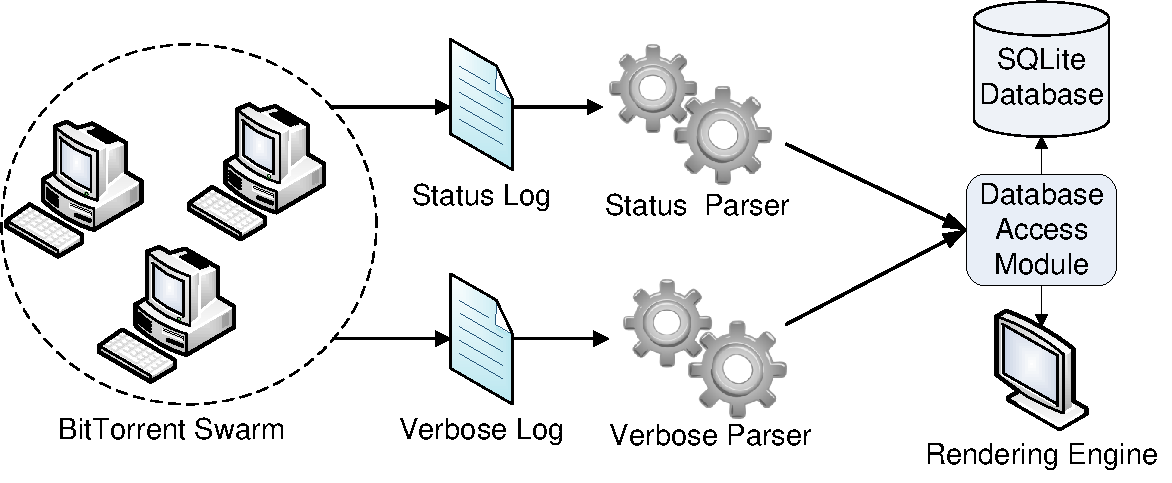
\includegraphics[width=0.7\textwidth]{src/img/proto-measure/logarch-not-use}
  \end{center}
  \caption{Structura sistemului de jurnalizare}
  \label{fig:proto-measure:logarch}
\end{figure}

Așa cum se poate observa în Figura~\ref{fig:proto-measure:logarch},
mesajele sunt trimise, folosind parsere specifice pentru fiecare tip de fișier
de jurnalizare, către modulul \textit{Database Access} care le stochează
într-o bază de date SQLite. Pentru a analiza comportamentul partenerilor,
modulul \textit{Rendering Engine} citește datele stocate folosind modulul
\textit{Database Access} și le afișează într-o interfață grafică.

Frameworkul de post-procesare este folosit pentru a stoca informațiile de
jurnalizare furnizate de diverși clienți de BitTorrent într-o zonă de stocare
(de obicei o bază de date). O perspectivă arhitecturală a platformei este
descrisă în Figura~\ref{fig:proto-measure:ppf-architecture}.

\begin{figure}[h]
  \begin{center}
    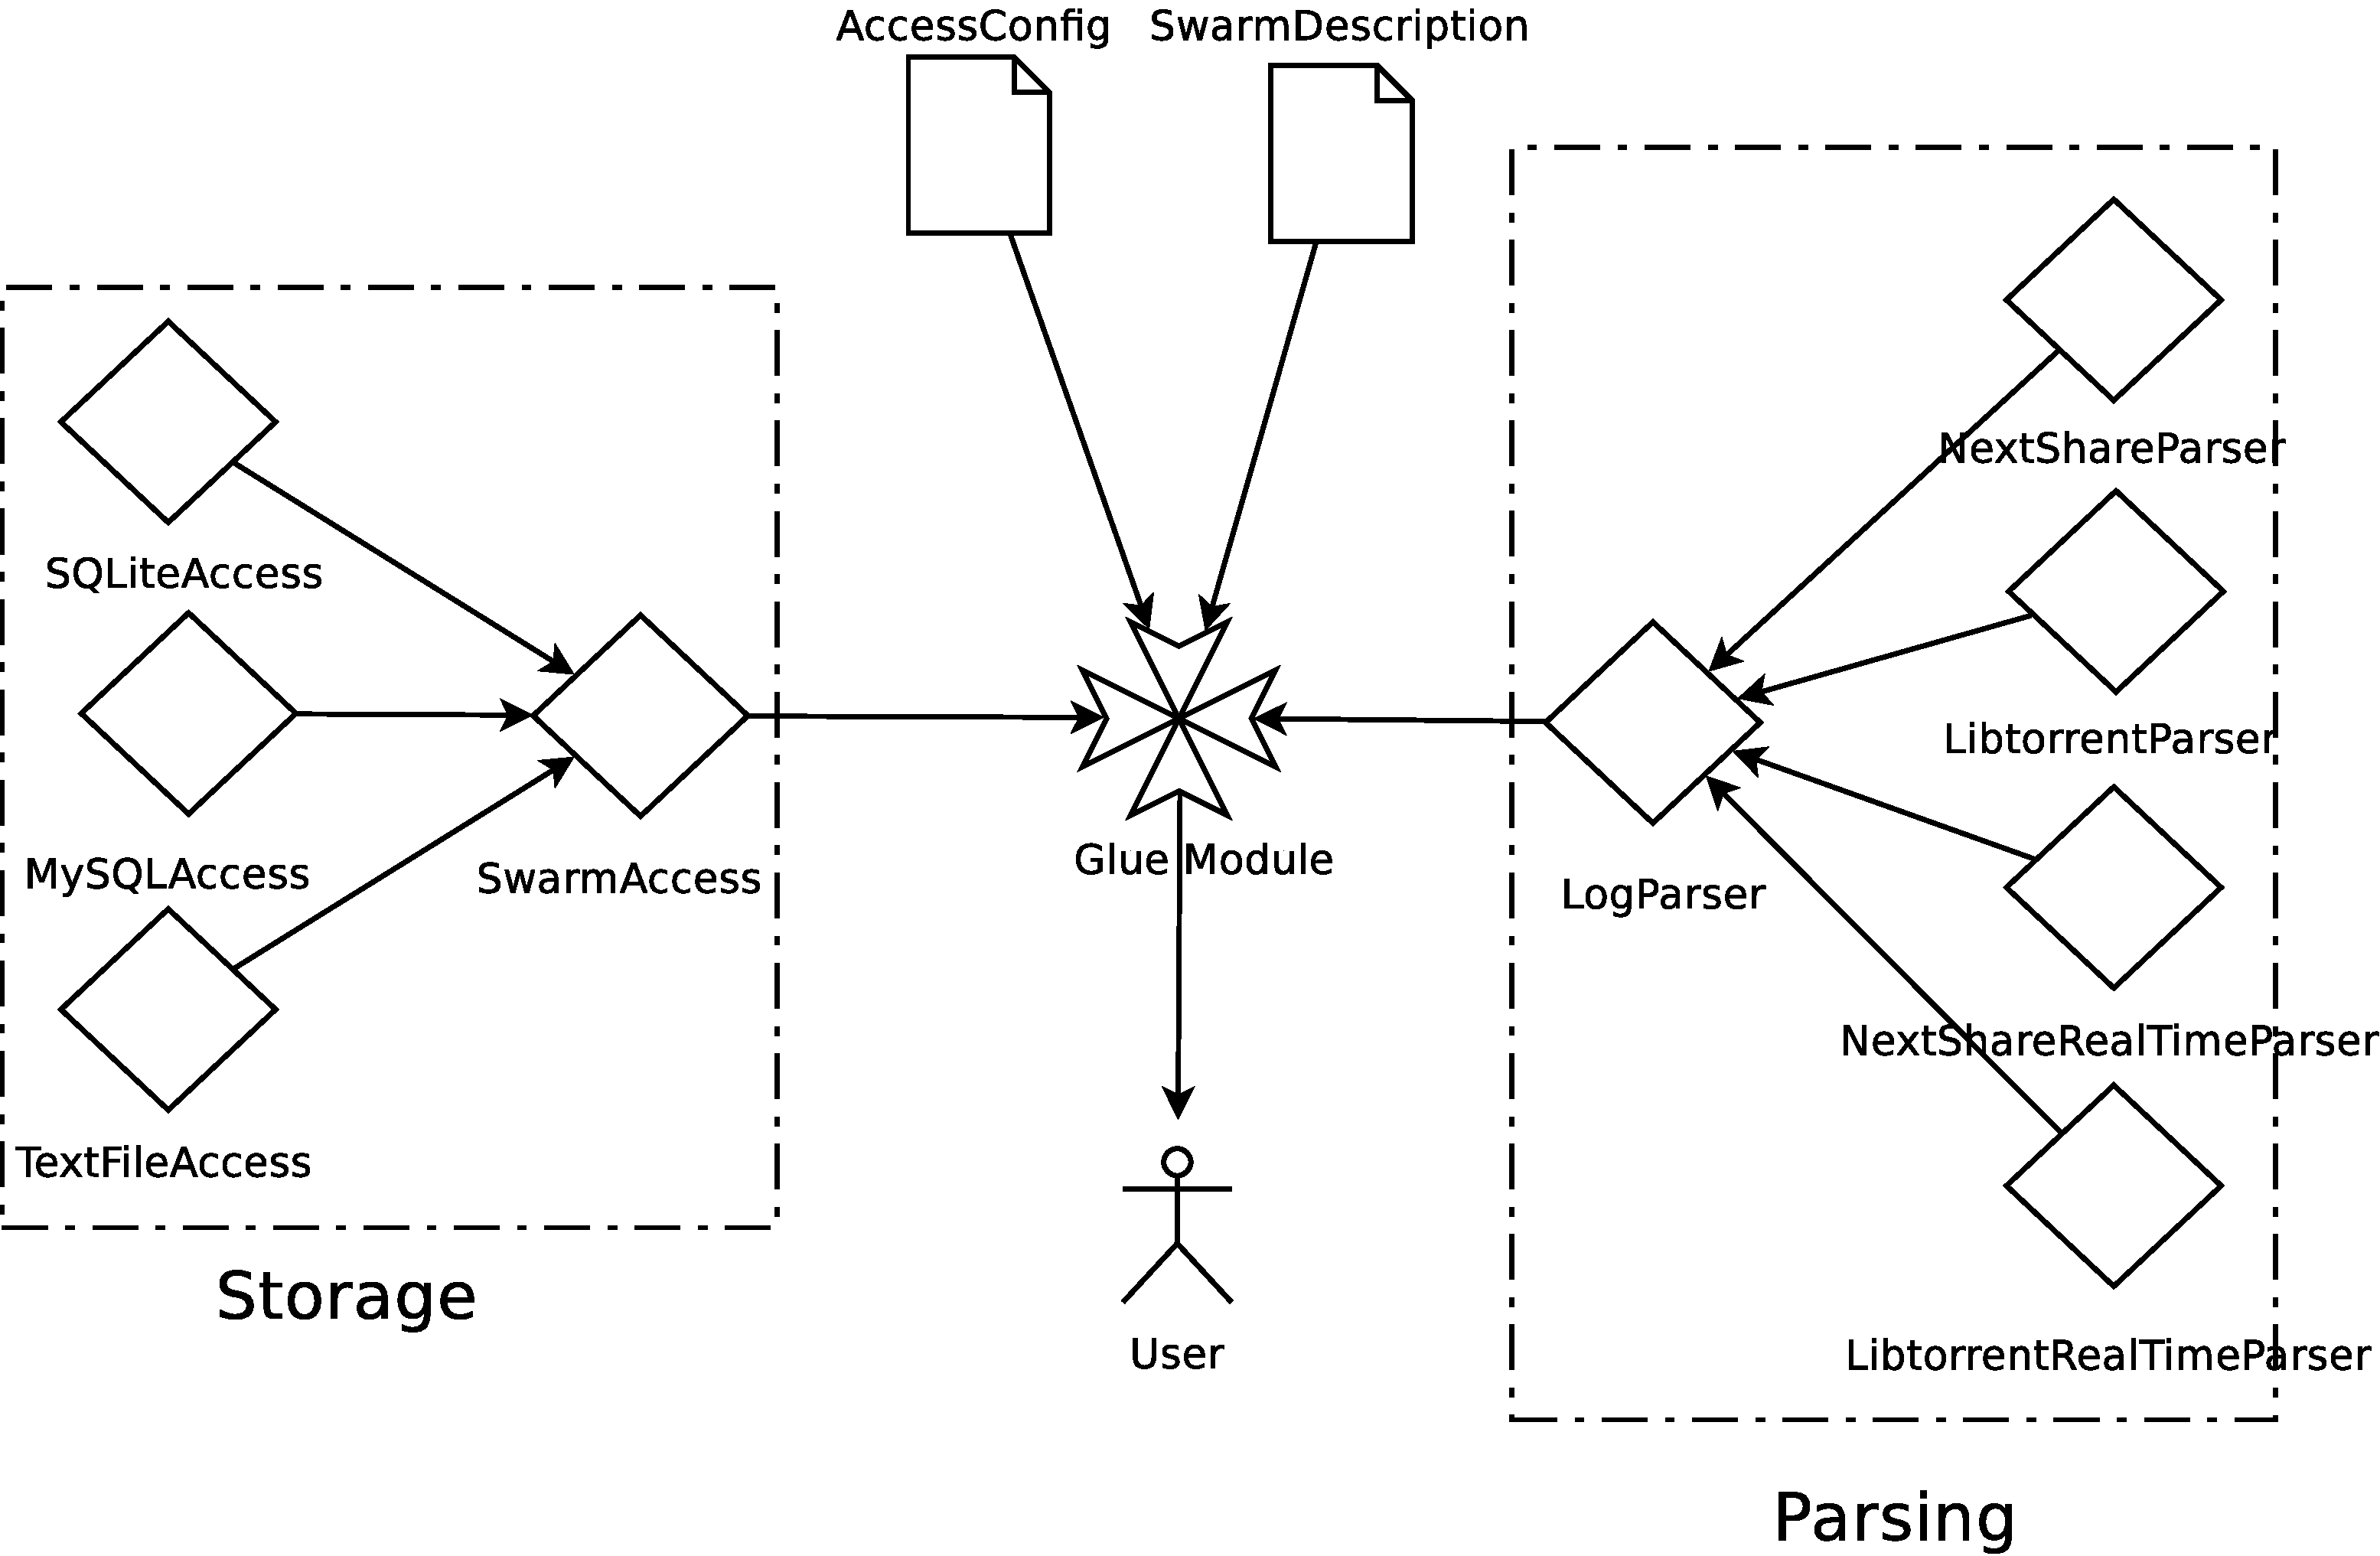
\includegraphics[width=0.7\textwidth]{src/img/proto-measure/ppf-architecture}
  \end{center}
  \caption{Arhitectura frameworkului de post-processing}
  \label{fig:proto-measure:ppf-architecture}
\end{figure}

Cele două componente principale ale frameworkului sunt parserul și componentele
de stocare. Parserele procesează informația de jurnalizare și extrag parametrii
protocolului care au fost măsurați pentru a fi supuși analizei; componentele
de stocare furnizează o interfață pentru stocarea în baza de date sau în fișiere
-- atât pentru scriere cât și pentru citire. Astfel, se oferă o interfață
ușor de accesat, rapidă și flexibilă. Aceste componente sunt invocate când
se face parsarea mesajelor -- pentru stocarea parametrilor, și pentru
analiza acestora -- pentru recuperarea/citirea/accesarea parametrilor.

\section{Evaluarea bazată pe măsurători de protocoale Peer-to-Peer}
\label{sec:proto-measure:eval-swarm}

Infrastructura de virtualizare și framework-ul automatizat furnizează
platforma necesară pentru evaluarea implementărilor Peer-to-Peer și a
modelelor formale. Interesul nostru este acela de evaluare a clienților
BitTorrent, interes care se traduce în viteză de download brută; cu cât este
viteza de download mai mare, cu atât performanța este mai bună. În mod
evident, trebuie să avem în vedere atât viteza de download a peer-ilor cât și
a swarm-ului. Un peer cu o viteză de downloa ridicată dar care nu este
altruist nu este binevenit într-un swarm dat.

Pentru o evaluare formală vom considera viteza de download ca unitatea de
evaluare a performanței. Considerăm celelalte unități măsurabile că sunt în
corelație cu viteza de download.

Diverse surse de variație influențează unitățile măsurate. Deși ne vom
concentra pe viteza de download, celelalte unități influențează de asemenea.
Dacă un peer primește un plus la viteza sa de upload atunci va fi mărită
viteza de download a altor peeri. Dacă o unitate influențează viteza de
upload, atunci aceasta va influența viteza de download, deși poate nu direct.
Este, posibil, mai ușor să se detecteze influența diversele unități pe
elemente secundare, precum mesajele de protocol.

Prin urmare, considerăm o corespondență între unitățile care variază și
unitățile măsurate.

\begin{align}
\label{eq:proto-measure:eval}
Eval(hw, sys, impl, swarm, net) = (protomsg, speed, conn, ruse)
\end{align}

Obiectivul nostru este maximizarea vitezei de download. Acesta se traduce în
definirea și ajustarea celor mai potrivite valor pentru unitățile care
variază. O implementare corespunzătoare, lansată întrun mediu corespunzător va
asigura o performanță ridicată.

Dacă vom continua să monitorizăm viteza de download, o formulă pur matematică
pentru un peer dat va fi.
\begin{align}
  FS = \int_0^{DT} DS(t)\,dt
\end{align}

unde:

\begin{itemize}
  \item FS (\textit{file size}) -- dimensiunea fișierului
  \item DT (\textit{download time}) -- timpul de download
  \item DS (\textit{download speed} -- viteza de download
\end{itemize}

Întrucât ne propunem să monitorizăm un peer periodic, formula se traduce în:

\begin{align}
  FS = \sum_{t=0}^{DT} DS_{t}
\end{align}

Aceasta furnizează corelarea necesară între evoluția vitezei de download și
timpul de download, atunci când se cunoaște dimensiunea fișierului.

Pentru a corela viteza de download cu alte unități, trebuie să considerăm
viteza de download ca interacțiunea cu alți peeri. Un peer poate descărca doar
dacă alți peeri încarcă. Formalizăm acest lucru prin intermediul unei matrice
care poate fi construită pentru fiecare interval (perioadă) de monitorizare:

\begin{align}
  PDS_{t} =
  \begin{pmatrix}
    ds_{1,1} = 0 & ds_{1,2} & \cdots & ds_{1,NP} \\
    ds_{2,1} & ds_{2,2} = 0 & \cdots & ds_{2,NP} \\
    \vdots & \vdots & \ddots & \vdots \\
    ds_{NP,1} & ds_{NP,2} & \cdots & ds_{NP,NP} = 0 \\
  \end{pmatrix}
\end{align}

unde:

\begin{itemize}
  \item $ds_{i,j}$ -- download speed of peer \texttt{j} from peer \texttt{i};
  \item \texttt{PDS} -- peer download speed matrix at time \texttt{t};
  \item \texttt{NP} -- number of peers in swarm;
\end{itemize}

Rezultă că matricea de upload este transpusa matricei de download. Viteza de
download a peer-ului $j$ de la peer-ul $i$ ($ds_{i,j}$) este egală cu viteza
de upload a peer-ului $i$ de la peer-ul $j$ ($us_{j,i}$). Adică:

\begin{align}
  PUS_{t} = PDS_{t}^{T}
\end{align}

Viteza de download instantă a unui peer este suma vitezelor de download din
transferul cu ceilalți peeri. În mod similar, viteza de upload a unui peer
este suma vitezelor de upload ale transferurilor de peeri. Cu alte cuvinte,
viteza de download instantanee a peer-ului $k$ ($DS_{k}$) este suma elementelor
din cadrul coloanei $k$ din matricea $PDS$, în vreme ce viteza de upload
instantanee a peer-ului $k$ ($US_{k}$) este suma elementelor de pe linia $k$
din matricea $PDS$ matrix. Adică:

\begin{align}
  DS_{k} = \sum_{i=1}^{NP} ds_{i,k}
\end{align}
\begin{align}
  US_{k} = \sum_{i=1}^{NP} ds_{k,i}
\end{align}

Trebuie ținut cont de faptul că matricea este un instrumet de raportare. Nu
furnizează o opțiune de configurare pentru funcționalitatea swarm-ului; este o
bază de date read-onlye care este actualizată pe măsură ce swarm-ul evoluează.
Evoluția peer-ilor și swarm-urilor este posibilă prin intermediul
interacțiunii dintre peeri, conexiunilor în rețea, disponibilității sau
limitării lățimii de bandă; acestea sunt punct de acțiune care au fost
îmbunătățite; matricea va putea oferi informații de raportare și, deci,
feedback referitor la actualizările aduse.
